% ===================================================================
% 文件名: tex/demo/main.tex
% 用途: TinyTeX 环境自检报告 (精简版 - 移除 newtx 字体依赖)
% ===================================================================

% [Group 2] 关键:强制指定 Fandol 字体,兼容 Windows Server
\PassOptionsToPackage{fontset=fandol}{ctex}

% [Group 1] 使用标准 article 类
\documentclass[a4paper, 12pt]{article}

% ===================================================================
% 0. 宏包加载区
% ===================================================================

% --- [Group 2] 中文支持 ---
\usepackage{ctex}      % 中文核心
\usepackage{zhnumber}  % 中文数字

% --- [Group 3] 字体与数学 (已修改) ---
\usepackage{iftex}     
\usepackage{amsmath, amsfonts, amssymb} 
\usepackage{esint}     

% 【修改点】注释掉了 newtx 字体包
% 移除了对 mweights, scalefnt, fontaxes, realscripts 的依赖
% \usepackage{newtxtext, newtxmath} 

% --- [Group 4] 模板逻辑 ---
\usepackage{appendix}  
\usepackage{abstract}  
\usepackage{hologo}    
\usepackage[stable]{footmisc} 
\usepackage{etoolbox}  

% --- [Group 5] 格式与功能 ---
\usepackage[margin=2.5cm]{geometry} 
\usepackage{xcolor}    
\usepackage{graphicx}  
\usepackage{mwe}       % 占位图
\usepackage{booktabs}  % 三线表
\usepackage{multirow}  
\usepackage{makecell}  
\usepackage{caption}   
\usepackage{subcaption}
\usepackage{enumitem}  
\usepackage{listings}  
\usepackage{fancyvrb}  
\usepackage{siunitx}   
\usepackage{microtype} 
\usepackage{tikz}      % 绘图
\usepackage[colorlinks=true, linkcolor=blue]{hyperref} 
\usepackage{cleveref}  

% --- [Group 5] 参考文献 (使用 biblatex + biber) ---
\usepackage[style=gb7714-2015, backend=biber]{biblatex}

% ===================================================================
% 1. 准备测试数据
% ===================================================================
\begin{filecontents}[overwrite]{ref.bib}
@manual{tinytex,
  title  = {TinyTeX Documentation},
  author = {Yihui Xie},
  year   = {2024},
  url    = {https://yihui.org/tinytex/}
}
@article{latex3,
  title   = {The LaTeX3 Interfaces},
  author  = {The LaTeX3 Project},
  journal = {TUGboat},
  year    = {2023}
}
\end{filecontents}
\addbibresource{ref.bib}

% TikZ 设置
\usetikzlibrary{shapes.geometric, arrows}

% 代码块设置
\lstset{
    basicstyle=\ttfamily\small,
    backgroundcolor=\color{gray!10},
    frame=single,
    keywordstyle=\color{blue}
}

% ===================================================================
% 正文开始
% ===================================================================
\title{\textbf{TinyTeX 环境自检报告 (无 NewTX)}}
\author{CI/CD Pipeline}
\date{\zhtoday}

\begin{document}

\maketitle

\begin{abstract}
    \noindent 
    本报告已移除 \texttt{newtxtext} 和 \texttt{newtxmath} 宏包,使用 LaTeX 默认字体(Computer Modern)。
    这消除了对底层字体工具(如 \texttt{scalefnt}, \texttt{mweights})的依赖,主要验证中文、绘图、表格及引用功能。
\end{abstract}

\tableofcontents
\vspace{1cm}

% -------------------------------------------------------------------
\section{核心环境与中文支持}
% -------------------------------------------------------------------
\subsection{编译引擎}
当前编译引擎为:
\ifxetex
    \textcolor{green!60!black}{\textbf{\hologo{XeTeX}}} (检测通过)
\else
    \textcolor{red}{\textbf{未知引擎}}
\fi

\subsection{中文与字体}
\begin{itemize}
    \item \textbf{基础中文}:汉字显示正常 (ctex + fandol)。
    \item \textbf{中文数字}:2025 -> \textbf{\zhnumber{2025}}。
    \item \textbf{字体样式}:\textit{楷体 Italic},\textbf{黑体 Bold}。
\end{itemize}

% -------------------------------------------------------------------
\section{数学公式 (Default Font)}
% -------------------------------------------------------------------
测试默认数学字体:
\begin{equation}
    \label{eq:maxwell}
    \oint_{\partial \Omega} \mathbf{E} \cdot d\mathbf{l} = -\frac{d}{dt} \iint_S \mathbf{B} \cdot d\mathbf{S}
\end{equation}
智能引用测试:\Cref{eq:maxwell}。

% -------------------------------------------------------------------
\section{多媒体与绘图}
% -------------------------------------------------------------------
\subsection{智能子图 (mwe + subcaption)}
\begin{figure}[htbp]
    \centering
    \begin{subfigure}{0.45\textwidth}
        \includegraphics[width=\linewidth]{example-image-a}
        \caption{Image A}
    \end{subfigure}
    \hfill
    \begin{subfigure}{0.45\textwidth}
        \includegraphics[width=\linewidth]{example-image-b}
        \caption{Image B}
    \end{subfigure}
    \caption{子图测试}
\end{figure}

\subsection{矢量绘图 (TikZ)}
\begin{center}
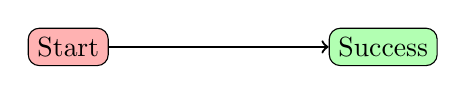
\begin{tikzpicture}
    \node (start) [rectangle, rounded corners, draw=black, fill=red!30] {Start};
    \node (end) [rectangle, rounded corners, draw=black, fill=green!30, right of=start, node distance=4cm] {Success};
    \draw [->, thick] (start) -- (end);
\end{tikzpicture}
\end{center}

% -------------------------------------------------------------------
\section{复杂表格与代码}
% -------------------------------------------------------------------
\subsection{专业表格}
\begin{table}[htbp]
    \centering
    \caption{安装状态表}
    \begin{tabular}{llc}
        \toprule
        \textbf{组件} & \textbf{关键包} & \textbf{状态} \\
        \midrule
        Tools & latexmk & OK \\
        Chinese & ctex & OK \\
        \bottomrule
    \end{tabular}
\end{table}

\subsection{代码高亮}
\begin{lstlisting}[language=TeX, caption=LaTeX Code]
% 物理单位测试
Speed: \qty{2.99e8}{\meter\per\second}
\end{lstlisting}

% -------------------------------------------------------------------
\section{引用测试}
% -------------------------------------------------------------------
本文使用了 TinyTeX\cite{tinytex} 进行构建。
\printbibliography[heading=bibintoc, title=参考文献]

\appendix
\section{附录测试}
附录内容正常显示。

\end{document}